\section{Strange metal phase in disordered MATBG: Quantum chaos and information scrambling}
%----------------------------------------------------------------------------------------
\begin{frame}{Magic-angle twisted bilayer graphene}
\begin{columns}
\begin{column}{0.6\textwidth}
\begin{block}{}
MATBG flatbands + interaction \\ $\implies$ superconductor + correlated insulator\footnote[frame]{\cite{cao2018unconventional}}
\end{block}

\begin{block}{}
Kagome flatbands + interaction + uncorrelated disorder \\ $\implies$ SYK physics%\footnote[frame]{\cite{wei2021optical}}
\end{block}

\begin{block}{}
MATBG flatbands + interaction + uncorrelated disorder \\ $\implies$ ?
\end{block}
\end{column}

\begin{column}{0.3\textwidth}
\begin{figure}
    \centering
    \begin{minipage}{\linewidth}
        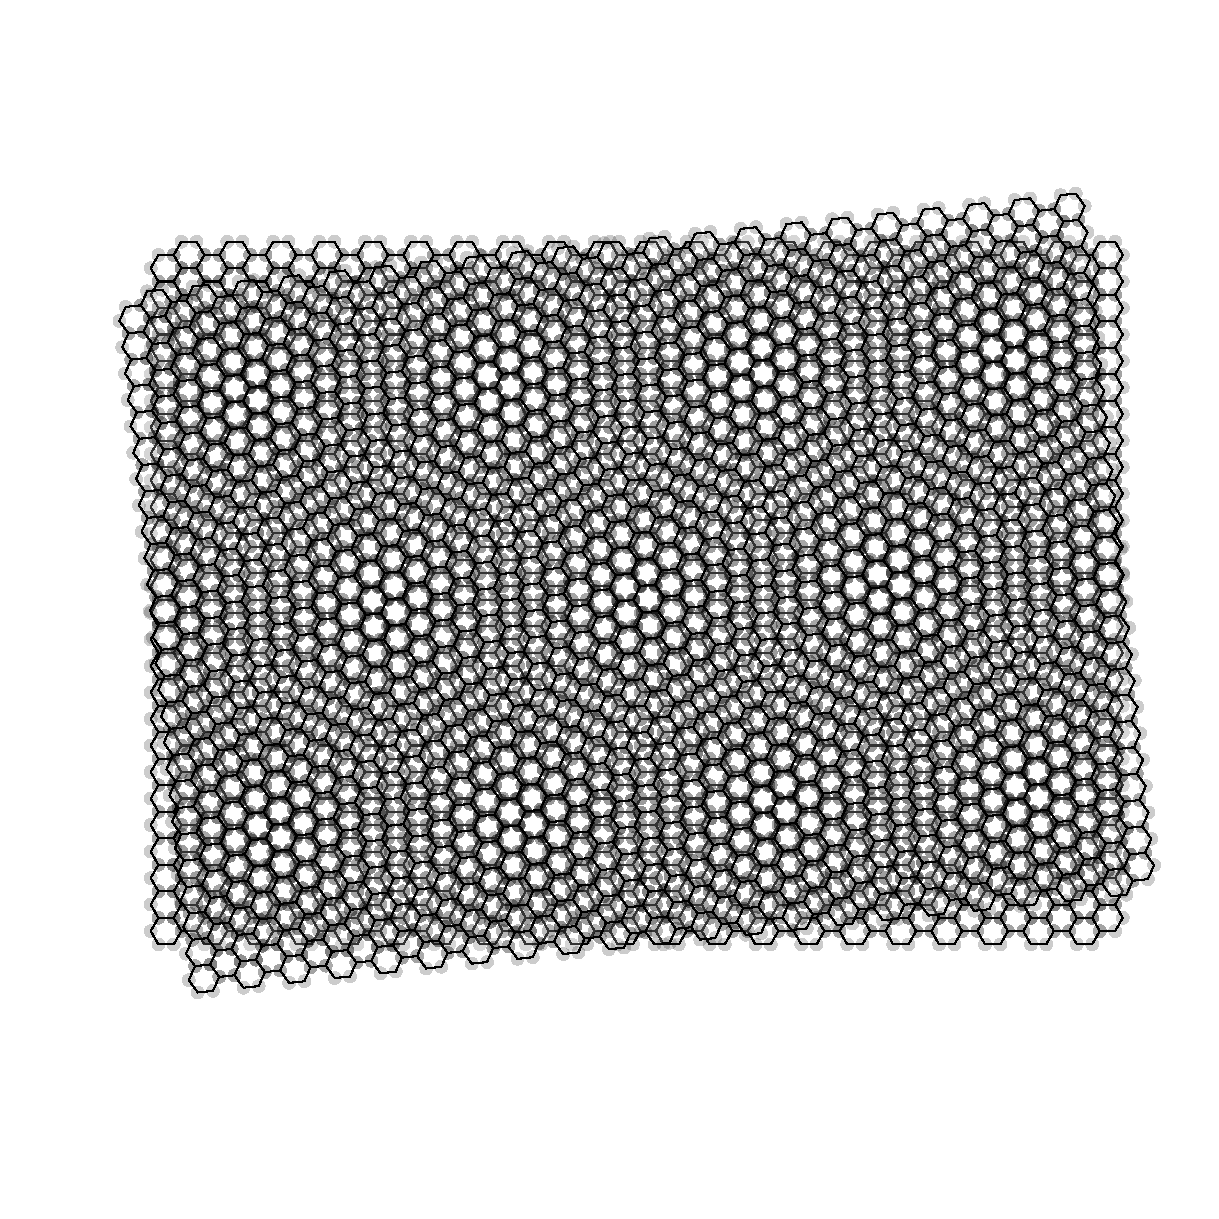
\includegraphics[width=0.75\textwidth]{figs/SM/morie.pdf}
    \end{minipage}
    \begin{minipage}{\linewidth}
        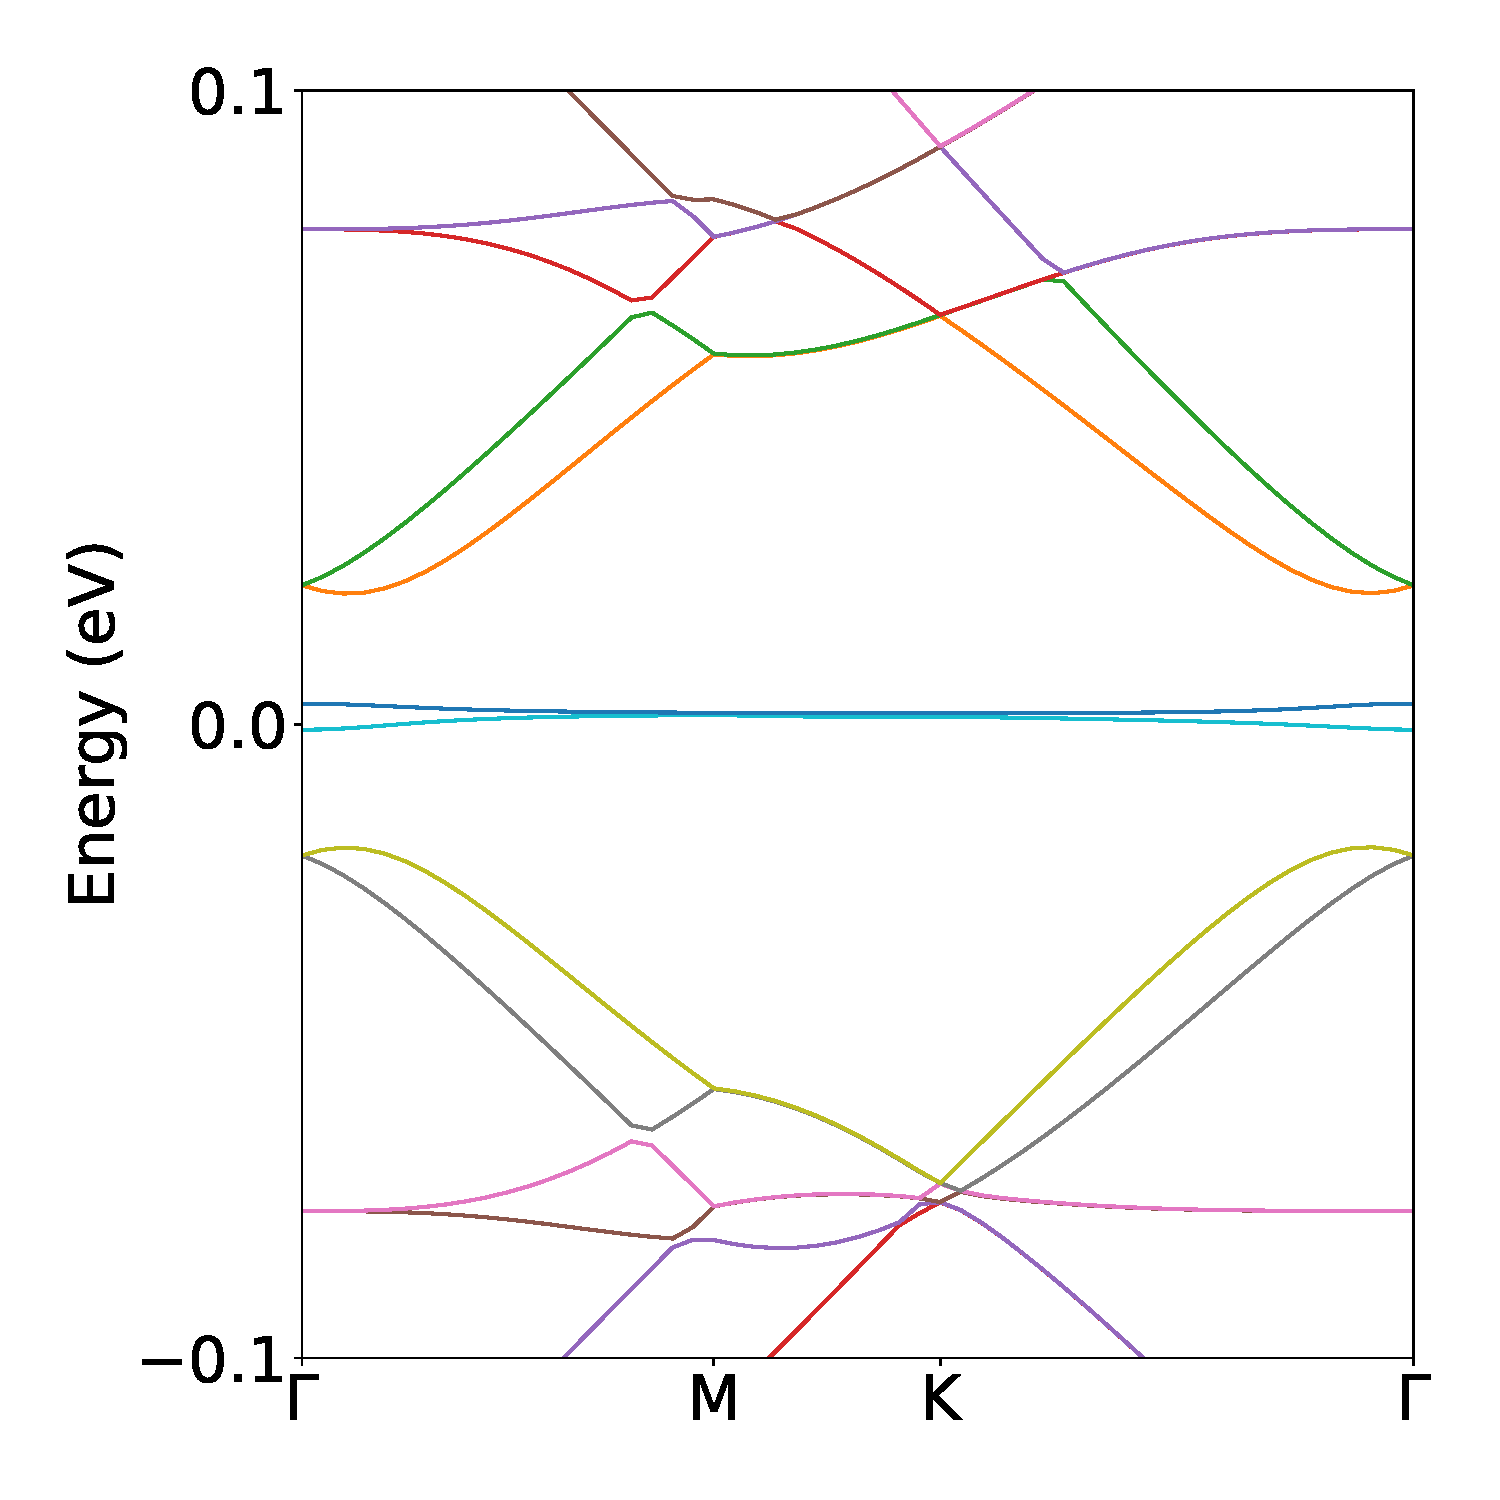
\includegraphics[width=0.75\textwidth]{figs/SM/FlatBand.pdf}
    \end{minipage}
\end{figure}
\end{column}
\end{columns}
\end{frame}
%----------------------------------------------------------------------------------------
\subsection{Weakly coupled SYK bundles}
%----------------------------------------------------------------------------------------
\begin{frame}{Tight Binding Model}
% \begin{equation*} \label{tight}
% \begin{aligned}
%     H_{tt'} &= -\sum_{\langle \mathbf{r}, \mathbf{r}' \rangle, \sigma, \chi} t a^{\dagger}_{\sigma \chi}(\mathbf{r}) a_{\sigma \chi}(\mathbf{r}') \\
%     &\quad - \sum_{\mathbf{r}, \mathbf{r}' , \sigma, \chi} t' e^{-(\mathbf{r} - \mathbf{r}')^2 / r_c^2} a^{\dagger}_{\sigma \chi}(\mathbf{r}) a_{\sigma \bar{\chi}}(\mathbf{r}')
% \end{aligned}
% \end{equation*}

\begin{equation*}
    H = \eqnmarkbox[NavyBlue]{hoppings}{H_{tt'}}
    + \eqnmarkbox[OliveGreen]{disorder}{H_{\mu}}
    + \eqnmarkbox[WildStrawberry]{interaction}{H_{I}}
\end{equation*}
\annotate[yshift=1em]{above,left}{hoppings}{hoppings}
\annotate[yshift=1em]{above, right}{disorder}{disorder}
\annotate[yshift=1em]{above, right}{interaction}{interaction}

\begin{equation*}
\begin{aligned}
    H_{tt'} &= \eqnmarkbox[Plum]{NN}{-\sum_{\langle \mathbf{r}, \mathbf{r}' \rangle, \sigma, \chi} t a^{\dagger}_{\sigma \chi}(\mathbf{r}) a_{\sigma \chi}(\mathbf{r}')} \\
    &\quad \eqnmarkbox[RoyalPurple]{intralayer}{- \sum_{\mathbf{r}, \mathbf{r}' , \sigma, \chi} t' e^{-(\mathbf{r} - \mathbf{r}')^2 / r_c^2} a^{\dagger}_{\sigma \chi}(\mathbf{r}) a_{\sigma \bar{\chi}}(\mathbf{r}')}
\end{aligned}
\end{equation*}
\annotate[yshift=1em]{above, right}{NN}{interlayer nearest neighbor hoppings}
\annotate[yshift=-1em]{below, right}{intralayer}{intralayer hoppings}
\end{frame}
%----------------------------------------------------------------------------------------
\begin{frame}{Random potential and low-energy states}
\begin{columns}
\begin{column}{0.33\textwidth}
\begin{equation*}
    H = \eqnmarkbox[NavyBlue]{hoppings}{H_{tt'}}
    + \eqnmarkbox[OliveGreen]{disorder}{H_{\mu}}
    + \eqnmarkbox[WildStrawberry]{interaction}{H_{I}}
\end{equation*}
\annotate[yshift=1em]{above,left}{hoppings}{hoppings}
\annotate[yshift=1em]{above, right}{disorder}{disorder}
\annotate[yshift=1em]{above, right}{interaction}{interaction}

\begin{block}{}
\begin{equation*}
    H_{\mu} = -\sum_{\mathbf{r}, \sigma, \chi} \mu(\mathbf{r}) a^{\dagger}_{\sigma \chi}(\mathbf{r}) a_{\sigma \chi}(\mathbf{r})
\end{equation*}
\begin{equation*}
    \mu(\mathbf{r}) = \sum_i w_{i} e^{-(\mathbf{r} - \mathbf{r}_{i})^2/2\sigma^2}
\end{equation*}
\end{block}
\end{column}

\begin{column}{0.6\textwidth}
\begin{figure}
    \centering
    \begin{minipage}{0.45\linewidth}
    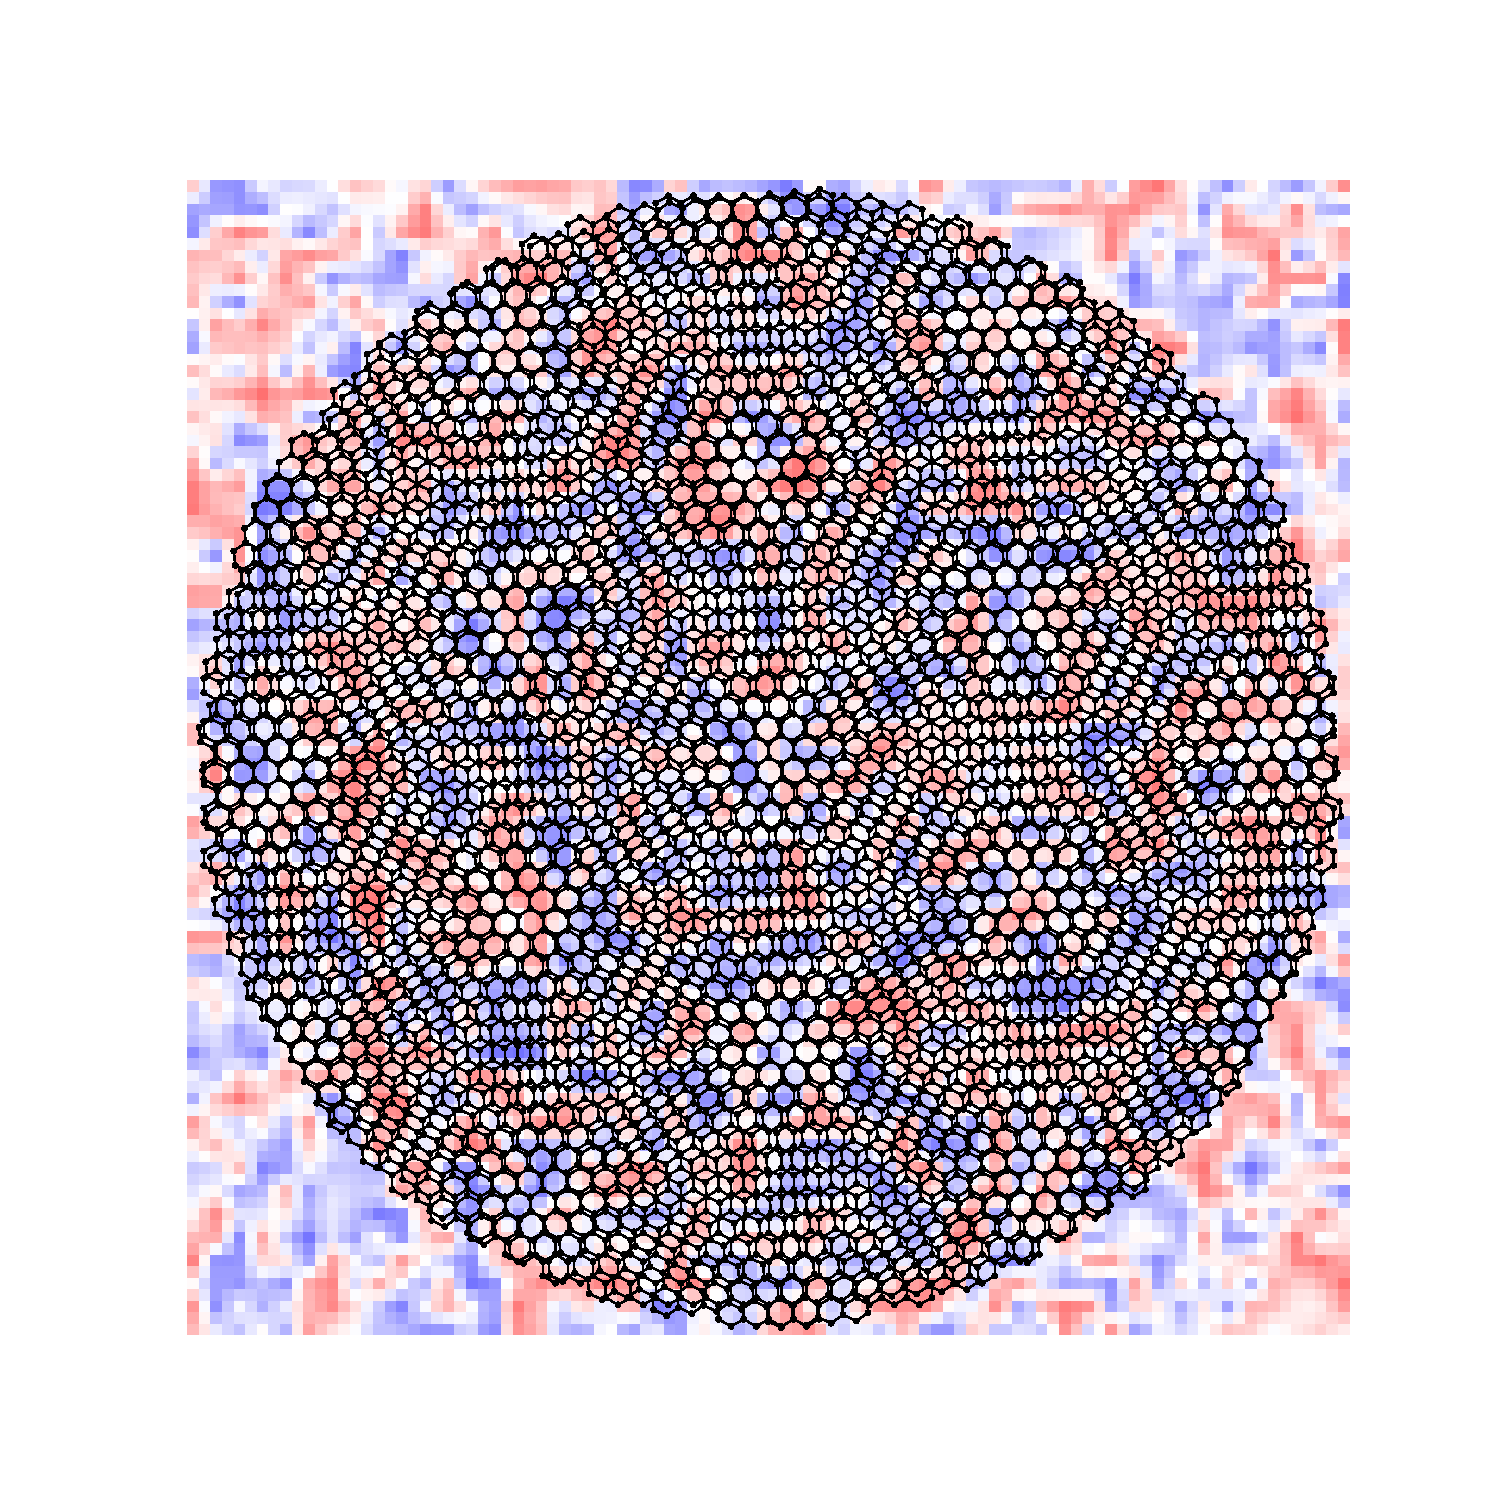
\includegraphics[width=\textwidth]{figs/SM/BLG.pdf}
    % \begin{picture}(0,0)
    % {\def\unitlength{} \put(0.1\textwidth,1.1\textwidth){$(b)$}}
    % \end{picture}
    % \phantomsubcaption{\label{TBG2}}
    \end{minipage}
    \begin{minipage}{0.45\linewidth}
    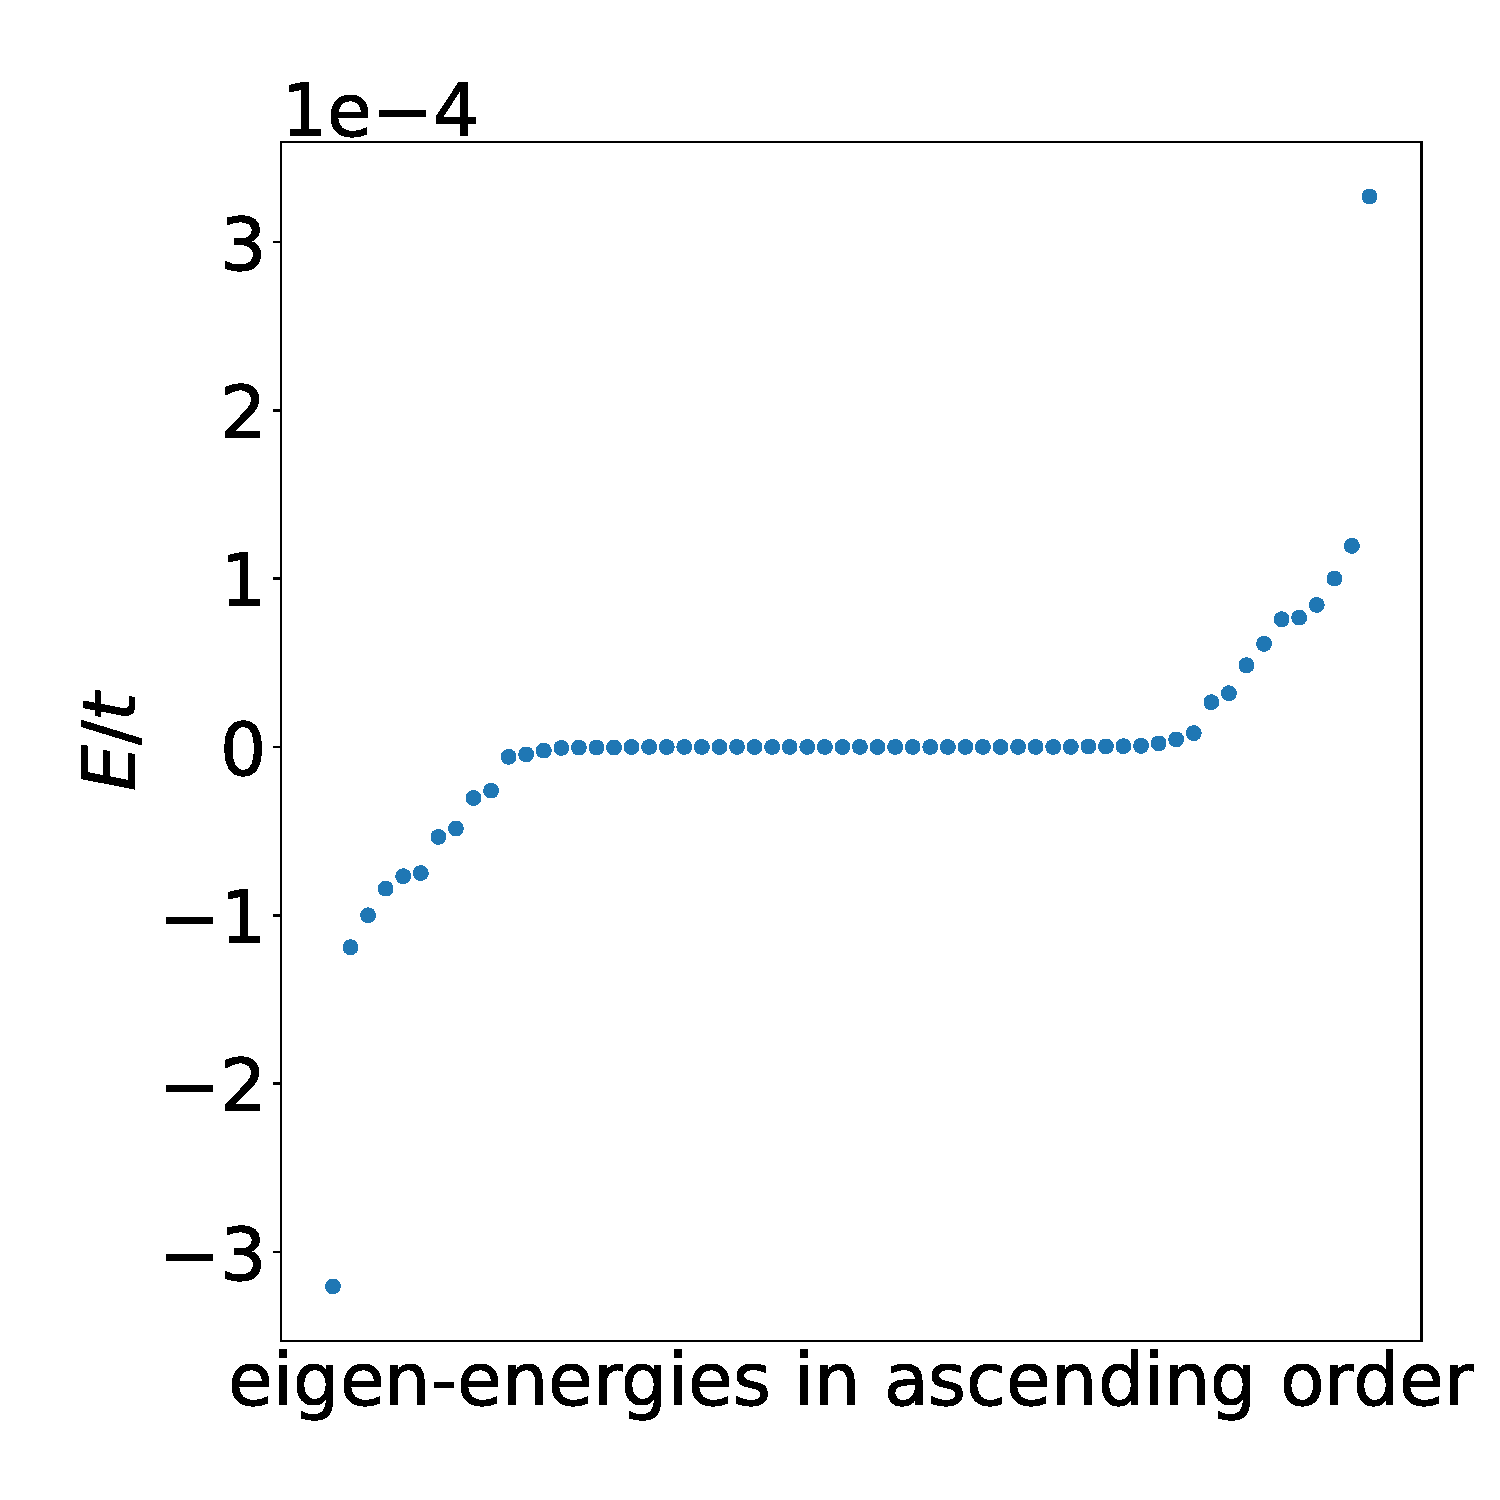
\includegraphics[width=\textwidth]{figs/SM/spectrum.pdf}
    % \begin{picture}(0,0)
    % {\def\unitlength{} \put(0.1\textwidth,1.1\textwidth){$(a)$}}
    % \end{picture}
    % \phantomsubcaption{\label{spectrum}}
    \end{minipage}
\end{figure}
\end{column}
\end{columns}
\end{frame}
%----------------------------------------------------------------------------------------
\begin{frame}{Weakly coupled SYK bundles}
\begin{columns}
\begin{column}{0.6\textwidth}
\begin{block}{}
    \begin{equation*}
    \begin{aligned}
        H_{I} = \sum_{\mathbf{r}, \mathbf{r}', \sigma, \chi, \sigma', \chi'} & \frac{1}{2} V_{\sigma, \chi, \sigma', \chi'}(\mathbf{r} - \mathbf{r}') \\
        \cross & a^{\dagger}_{\sigma \chi}(\mathbf{r}) a^{\dagger}_{\sigma' \chi'}(\mathbf{r}') a_{\sigma' \chi'}(\mathbf{r}') a_{\sigma \chi}(\mathbf{r})
    \end{aligned}
    \end{equation*}
    
    % \begin{equation*}
    %     V_{\sigma, \chi, \sigma', \chi'}(\mathbf{r} - \mathbf{r}') =
    %     \begin{cases}
    %         U, \quad \sigma = \bar{\sigma'}, \chi = \chi', \mathbf{r} = \mathbf{r}' \\
    %         V, \quad \chi = \chi', 0 < |\mathbf{r} - \mathbf{r}'| \leq a \\
    %         V, \quad \chi \neq \chi', 0 < |\mathbf{r} - \mathbf{r}' + \mathbf{d}| \leq a \\
    %         0, \quad \mathrm{otherwise}
    %     \end{cases}
    % \end{equation*}
\end{block}

\begin{block}{}
    \begin{equation*} \label{flatband}
        H_{\mathrm{int}} = \sum_{i<j,k<l} J_{ijkl} c_{i}^{\dagger} c_{j}^{\dagger} c_{k} c_{l}
    \end{equation*}
    
    \begin{equation*}
    \begin{aligned}
        J_{ijkl} = & \sum_{\mathbf{r}, \mathbf{r}', \sigma, \chi, \sigma', \chi'} V_{\sigma, \chi, \sigma', \chi'}(\mathbf{r} - \mathbf{r}') \\
        &\quad \cross \left[ \phi^*_{i; \sigma, \chi}(\mathbf{r}) \phi^*_{j; \sigma', \chi'}(\mathbf{r}') - \phi^*_{j; \sigma, \chi}(\mathbf{r}) \phi^*_{i; \sigma', \chi'}(\mathbf{r}') \right] \\
        &\quad \cross \left[ \phi_{k; \sigma', \chi'}(\mathbf{r}') \phi_{l; \sigma, \chi}(\mathbf{r}) - \phi_{l; \sigma', \chi'}(\mathbf{r}') \phi_{k; \sigma, \chi}(\mathbf{r}) \right]
    \end{aligned}
    \end{equation*}
\end{block}
\end{column}

\begin{column}{0.3\textwidth}
\begin{figure}
    \centering
    \begin{minipage}{\linewidth}
    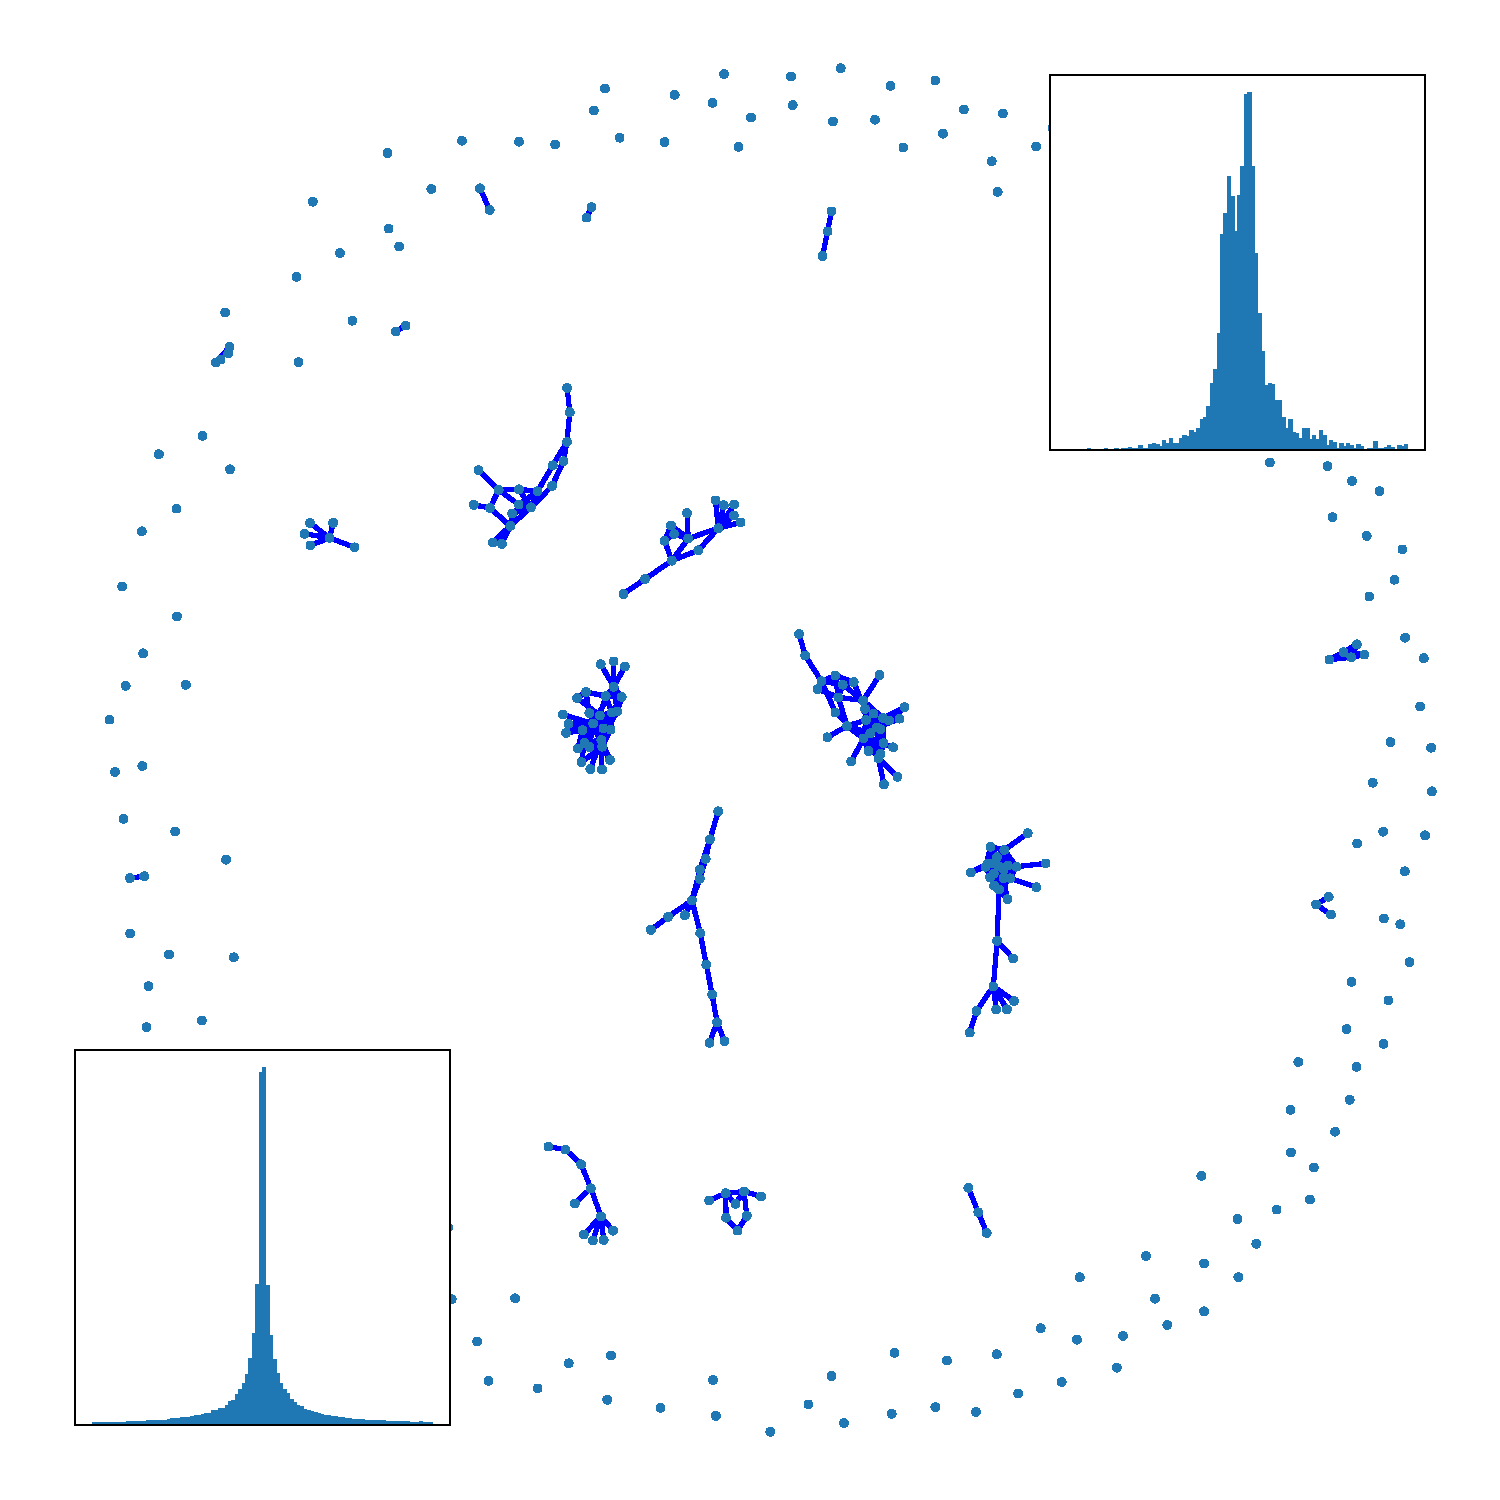
\includegraphics[width=\textwidth]{figs/SM/JTopo.pdf}
    \begin{picture}(0,0)
    {\def\unitlength{}
    % \put(-0.5\textwidth,\textwidth){$(b)$}
    \put(-0.05\textwidth,0.0\textwidth){$|J_{ijkl}|/\sigma_{\rm weak}$}
    \put(-0.04\textwidth,0.08\textwidth){$-1$}
    \put(0.28\textwidth,0.08\textwidth){$1$}
    \put(-0.05\textwidth,0.25\textwidth){$\rho$}
    \put(0.58\textwidth,0.65\textwidth){$|J_{ijkl}|/\sigma_{\rm strong}$}
    \put(0.61\textwidth,0.72\textwidth){$-3$}
    \put(0.93\textwidth,0.72\textwidth){$3$}
    \put(0.61\textwidth,0.9\textwidth){$\rho$}
    }
    \end{picture}
    % \phantomsubcaption{\label{JTopo}}
    \end{minipage}
\end{figure}
\end{column}
\end{columns}
\end{frame}
%----------------------------------------------------------------------------------------
\subsection{Thermodynamics}
%----------------------------------------------------------------------------------------
\begin{frame}{Thermodynamics}
\begin{columns}
\begin{column}{0.5\textwidth}
\begin{figure}
    \centering
    \begin{minipage}{0.49\linewidth}
    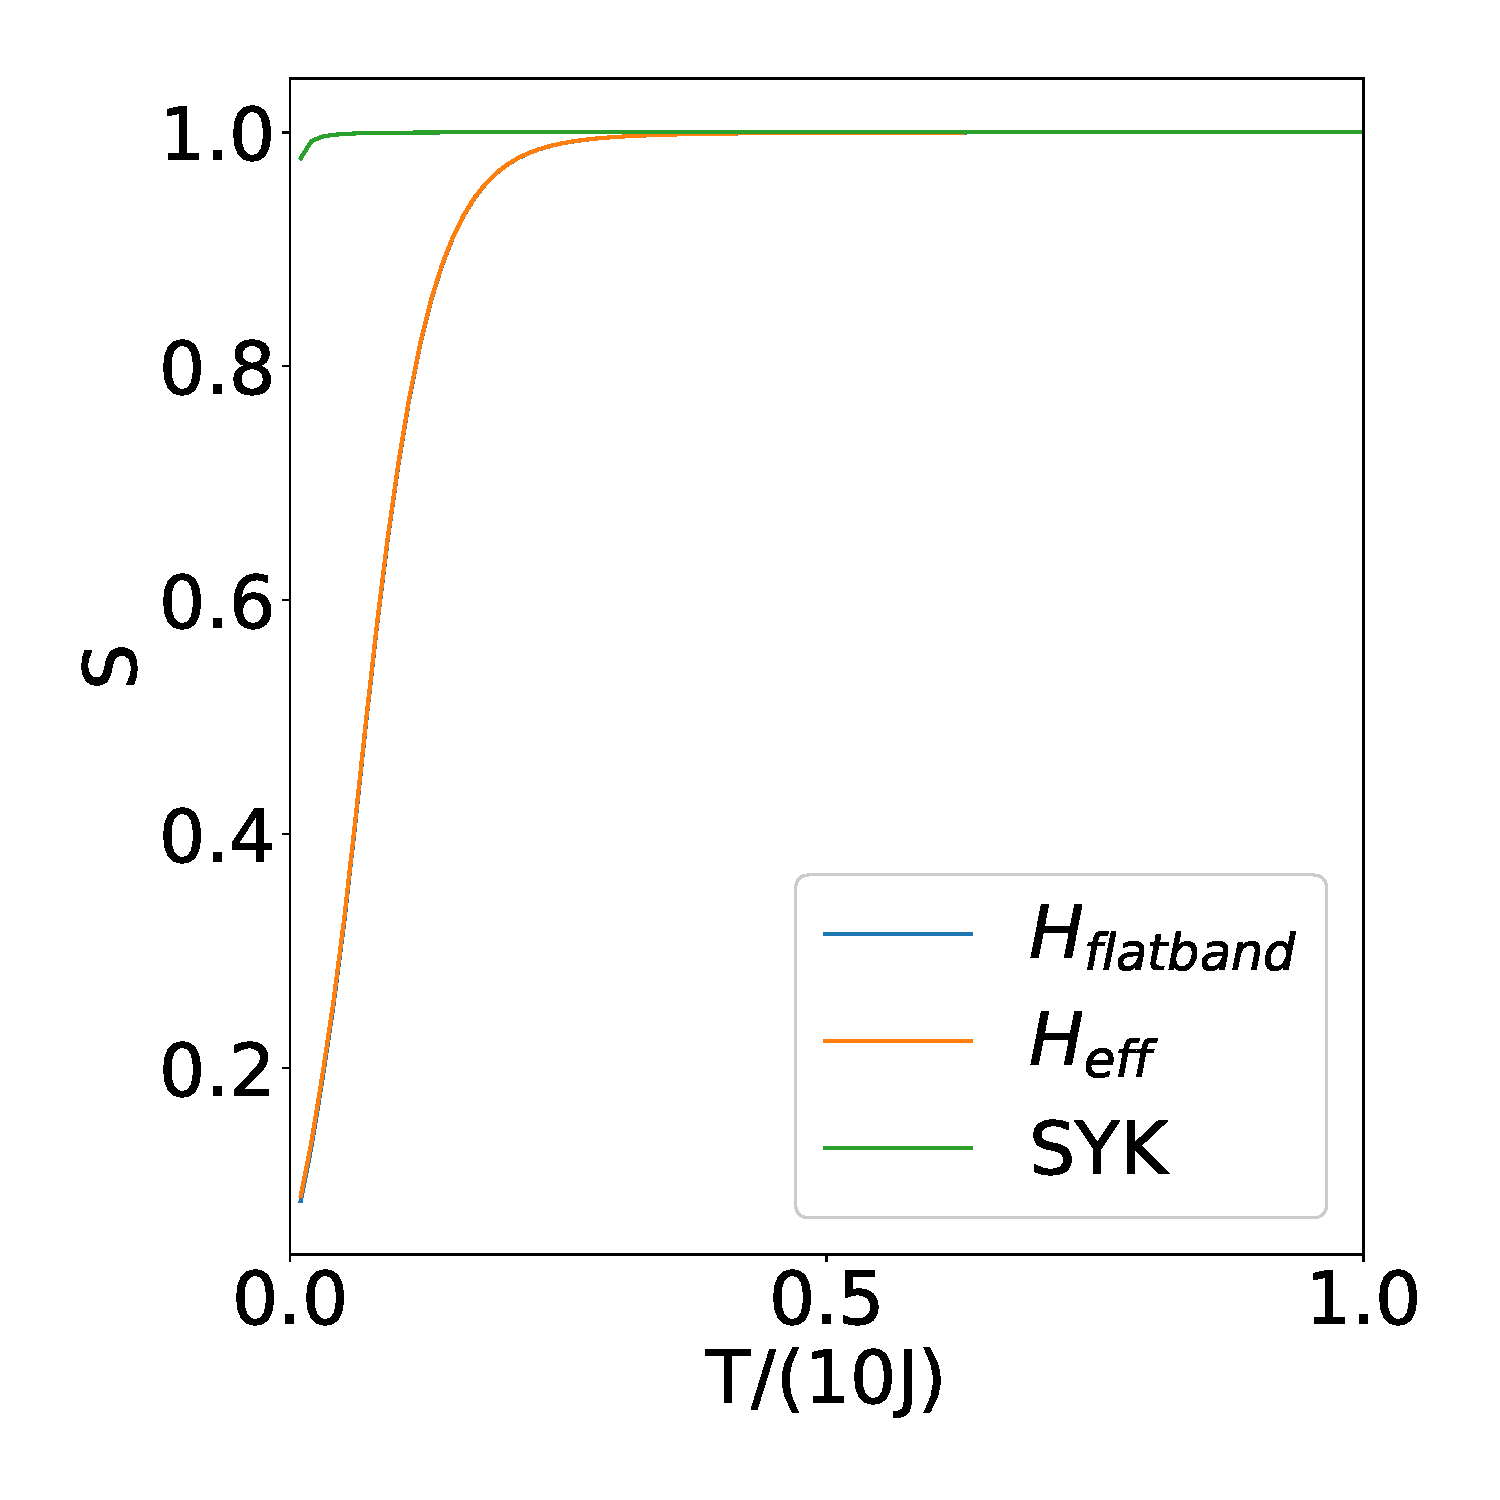
\includegraphics[width=\textwidth]{figs/SM/S.pdf}
    % \begin{picture}(0,0)
    % {\def\unitlength{} \put(0.1\textwidth,1.1\textwidth){$(c)$}}
    % \end{picture}
    % \phantomsubcaption{\label{entropy}}
    \end{minipage}
    \begin{minipage}{0.49\linewidth}
    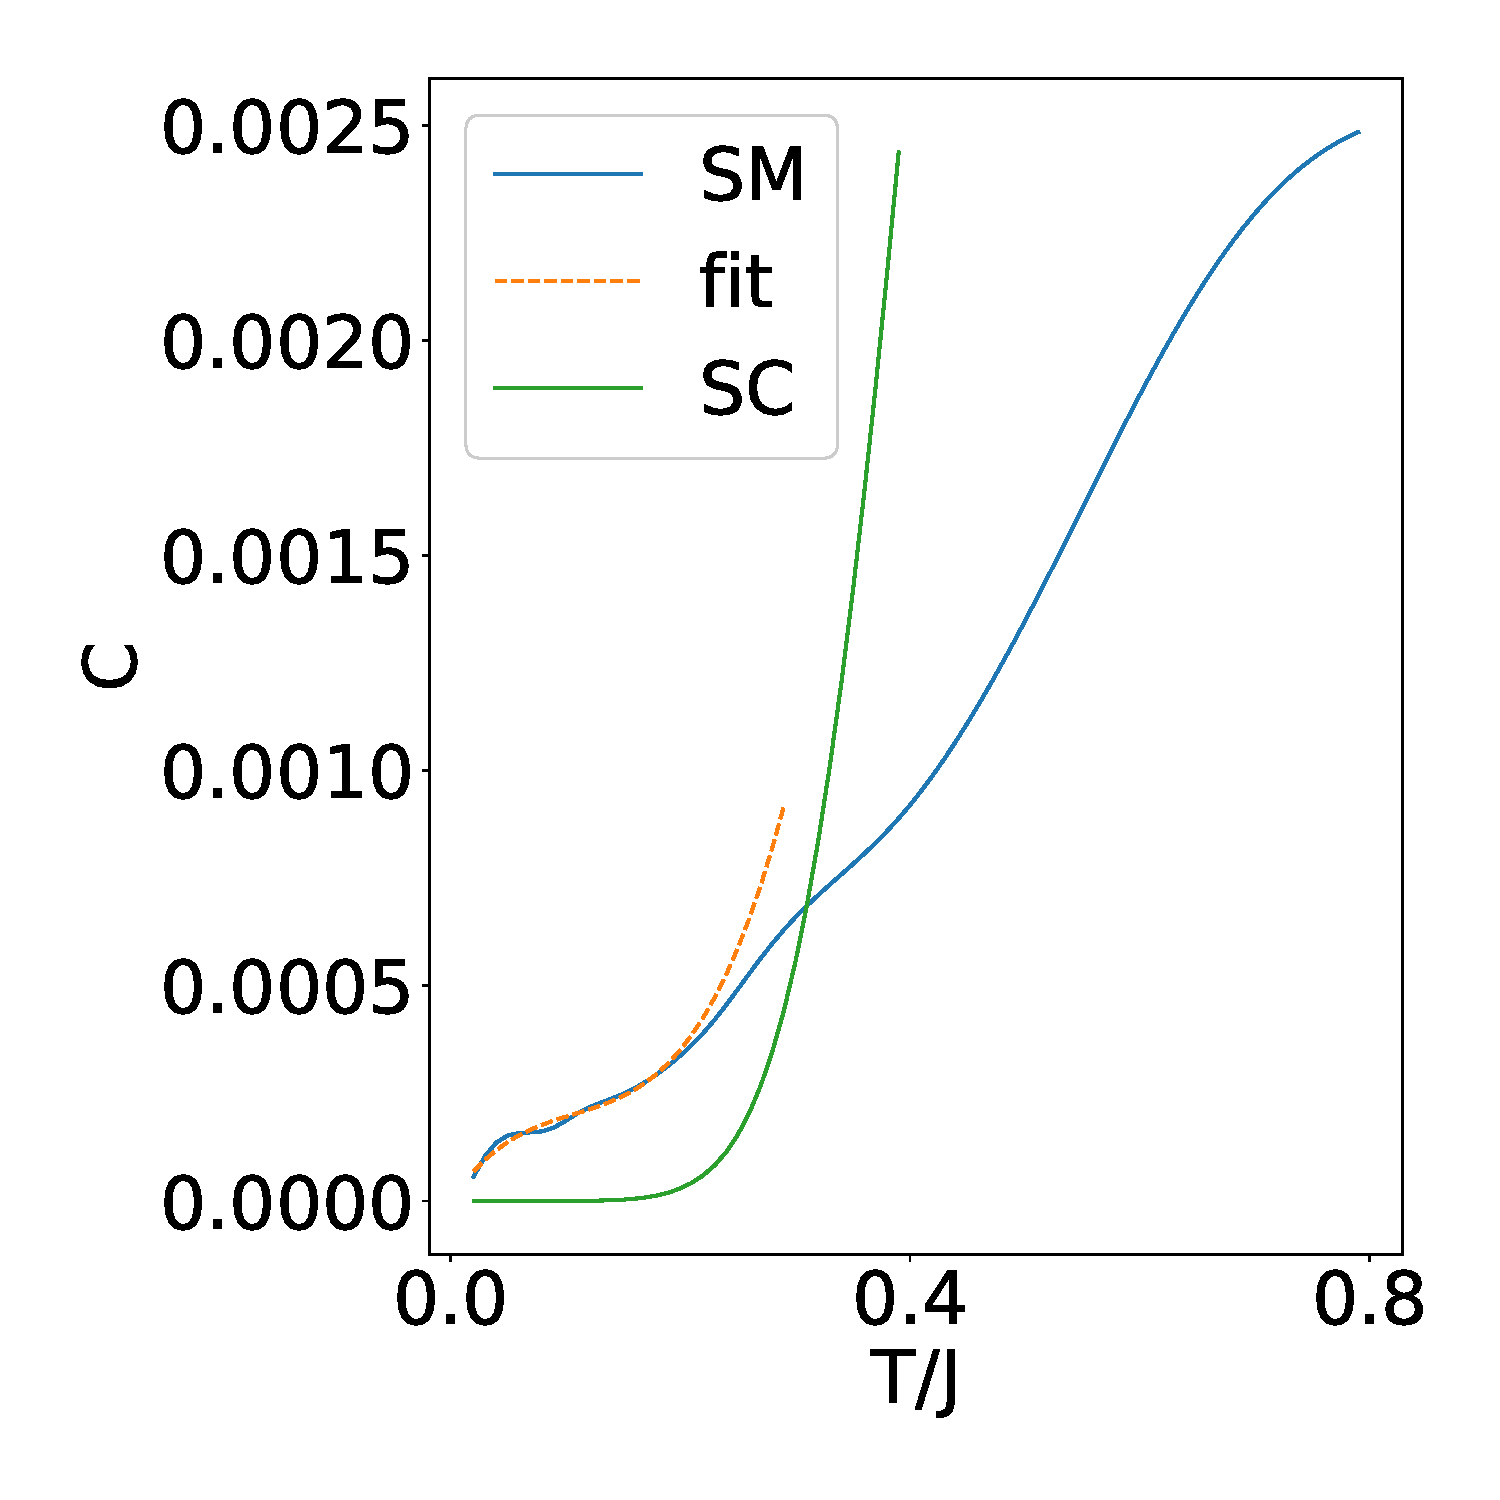
\includegraphics[width=\textwidth]{figs/SM/C_2.pdf}
    % \begin{picture}(0,0)
    % {\def\unitlength{} \put(0.1\textwidth,1.1\textwidth){$(d)$}}
    % \end{picture}
    % \phantomsubcaption{\label{capacity}}
    \end{minipage}
\end{figure}
\end{column}

\begin{column}{0.4\textwidth}
\begin{itemize}
    % \item Superconducting phase: $C_{SC} \sim e^{-T/\Delta}$

    \item SYK: $C_{SYK} \sim c_1 T + c_2 T^2 + c_3 T^3$

    \item The fitted $c_1 = 0.04$ is about one-tenth of the analytical and numerical results for the SYK model\footnote[frame]{\cite{maldacena2016comments,garcia2016spectral}}

    \item Normal phase of the superconductor: $C_{N} \sim T \ln(1/T)$\footnote[frame]{\cite{patel2022universal,michon2022planckian}}
\end{itemize}
\end{column}
\end{columns}
\end{frame}
%----------------------------------------------------------------------------------------
\subsection{Quantum chaos and information scrambling}
%----------------------------------------------------------------------------------------
\begin{frame}{Time reversal symmetry and GOE}
\begin{columns}
\begin{column}{0.6\textwidth}
\begin{figure}
    \centering
    \begin{minipage}{0.8\linewidth}
    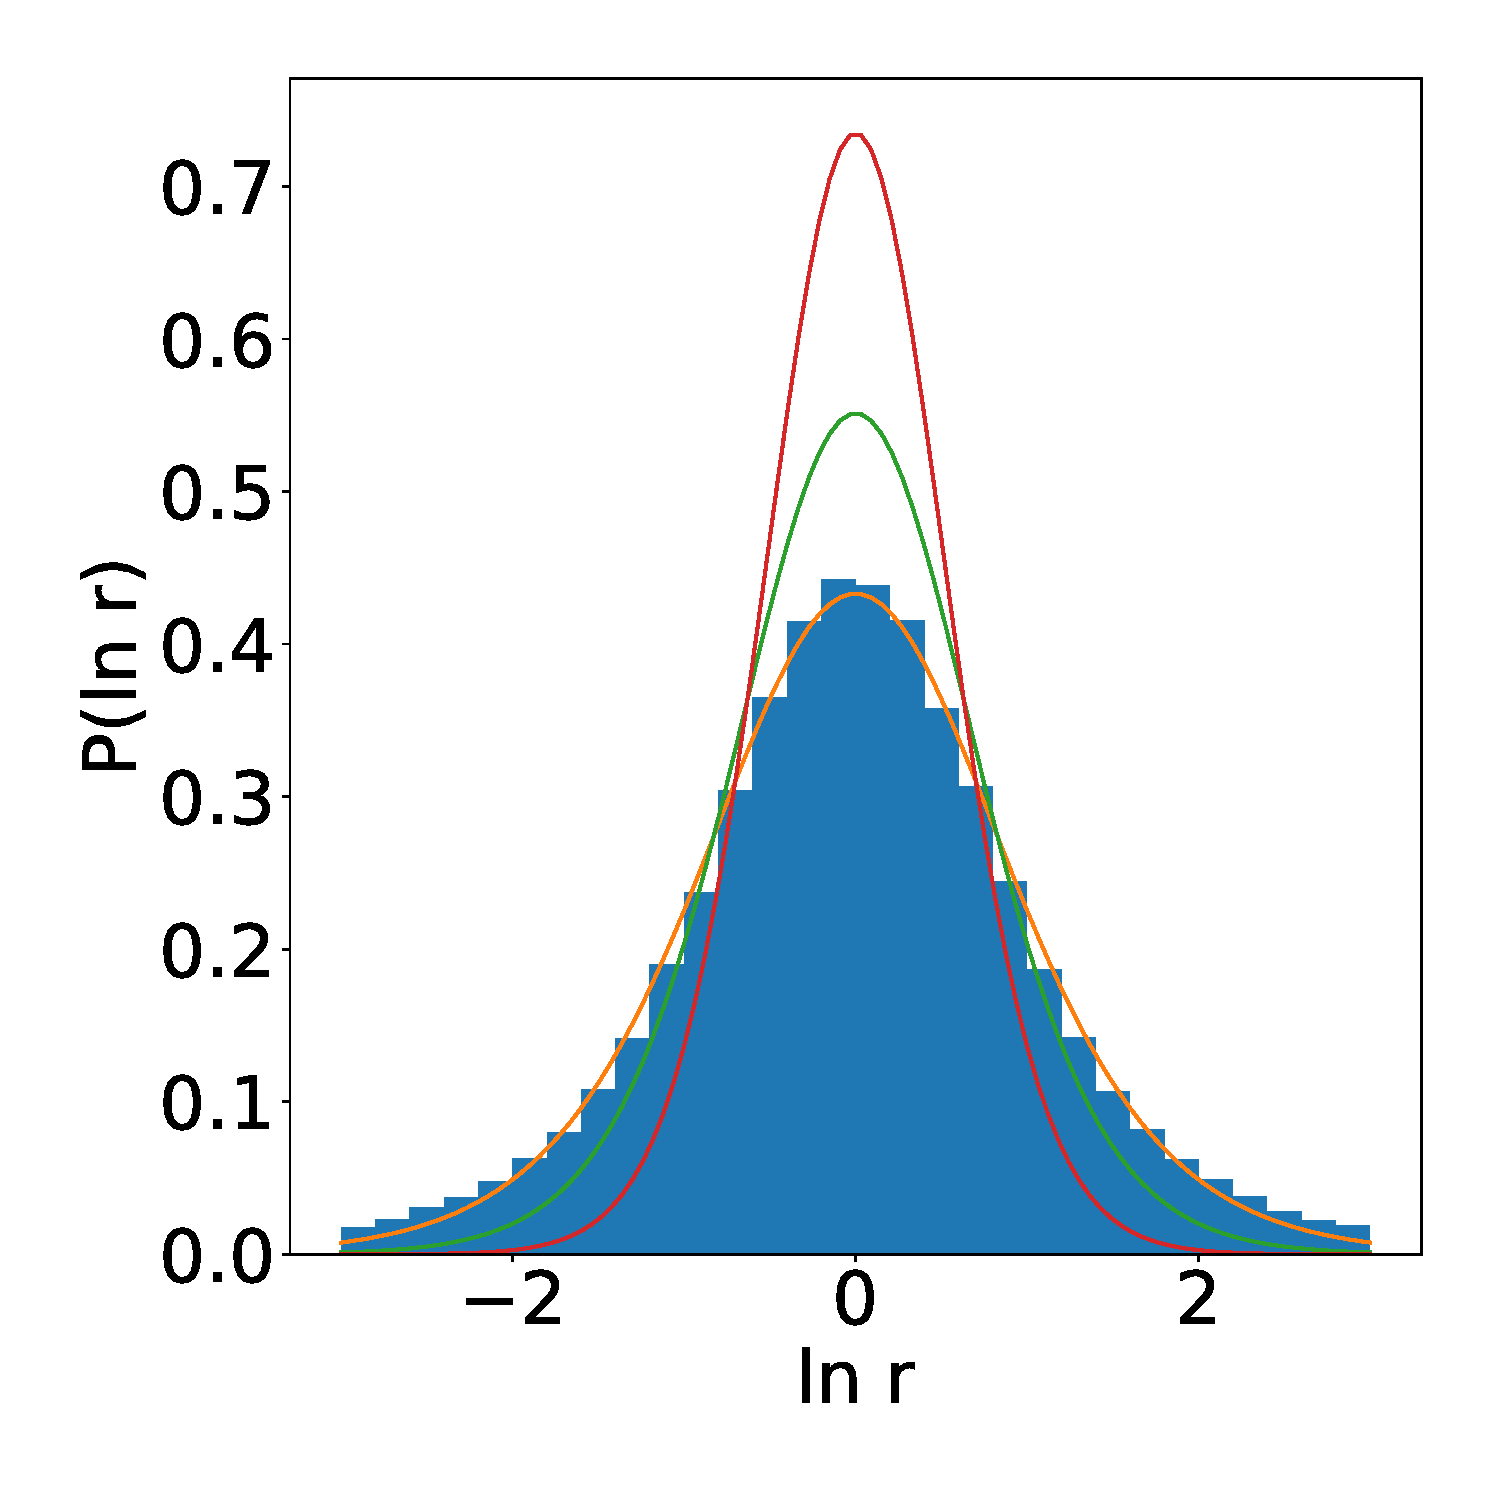
\includegraphics[width=\textwidth]{figs/SM/r.pdf}
    \begin{picture}(0,0)
    %{\def\unitlength{} \put(0.1\textwidth,1.1\textwidth){$(a)$}}
    % GXE labels
    {\def\unitlength{} \put(0.7\textwidth,0.78\textwidth){\text{\tiny GSE}}}
    {\def\unitlength{} \put(0.7\textwidth,0.8\textwidth){\vector(-1,0){18pt}}}
    {\def\unitlength{} \put(0.7\textwidth,0.68\textwidth){\text{\tiny GUE}}}
    {\def\unitlength{} \put(0.7\textwidth,0.7\textwidth){\vector(-1,0){17pt}}}
    {\def\unitlength{} \put(0.7\textwidth,0.58\textwidth){\text{\tiny GOE}}}
    {\def\unitlength{} \put(0.7\textwidth,0.6\textwidth){\vector(-1,0){16pt}}}
    % comment
    {\def\unitlength{} \put(0.21\textwidth,0.97\textwidth){\scriptsize Wigner-Dyson}
    {\def\unitlength{} \put(0.21\textwidth,0.92\textwidth){\scriptsize statistics}}}
    {\def\unitlength{} \put(0.21\textwidth,0.8\textwidth){$r_n = \frac{E_{n+1} - E_{n}}{E_{n} - E_{n-1}}$}}
    \end{picture}
    % \phantomsubcaption{\label{GEO}}
    \end{minipage}
\end{figure}
\end{column}

\begin{column}{0.3\textwidth}
\begin{itemize}
    \item RMT describes the quantum chaos in semi-classical and long time limit
    \item Non-chaotic level space behave like a Poisson process
\end{itemize}
\end{column}
\end{columns}
\end{frame}
%----------------------------------------------------------------------------------------
\begin{frame}{Lyapunov exponent and butterfly velocity}
\begin{columns}
\begin{column}{0.3\textwidth}
\begin{itemize}
\only<1>{
    \item Out-of-Time-Ordered Correlator:
    $\begin{aligned}[t]
        &OTOC \equiv \\
        &\langle X(x, \tau) Y(0) X(x, \tau) Y(0) \rangle_{\beta} \\
        &\sim - \langle [ X(x, \tau), Y(0) ]^2 \rangle_{\beta}
    \end{aligned}$
    
    \item $OTOC \sim -\left( \frac{\partial X(x, \tau)}{\partial Y(0)} \right)^2$ in semiclassical limit
    
    \item $OTOC \sim e^{\lambda (\tau - x/v_B)}$
}
\only<2>{
    \item Fermi liquid: $\lambda \sim T^2$ at low temperatures
    \item Maximal quantum chaos: $\lambda \sim T$\footnote[frame]{\cite{hartnoll2021planckian}} and $\lambda \le \lambda_{max}\equiv 2\pi T$\footnote[frame]{\cite{maldacena2016bound}}
    
    \item In the superconducting phase, $OTOC$ decays exponentially in $T$\footnote[frame]{\cite{larkin1969quasiclassical}}
}
\only<3>{
    \item For Fermi liquid with $\omega \sim k^z$, $v_B = \frac{d\omega}{dk} \sim \omega^{1-1/z} \sim T^{1-1/z}$
    % \item This argument fails for flatband non-FL
    \item $v_B \sim T^\delta$ $\delta > 1$ $\implies$ No quasiparticles
    \item $v_B$ describe the rate of quantum information scrambling
}
\end{itemize}
\end{column}

\begin{column}{0.6\textwidth}
\begin{figure}
    \centering
    \begin{minipage}{0.49\linewidth}
    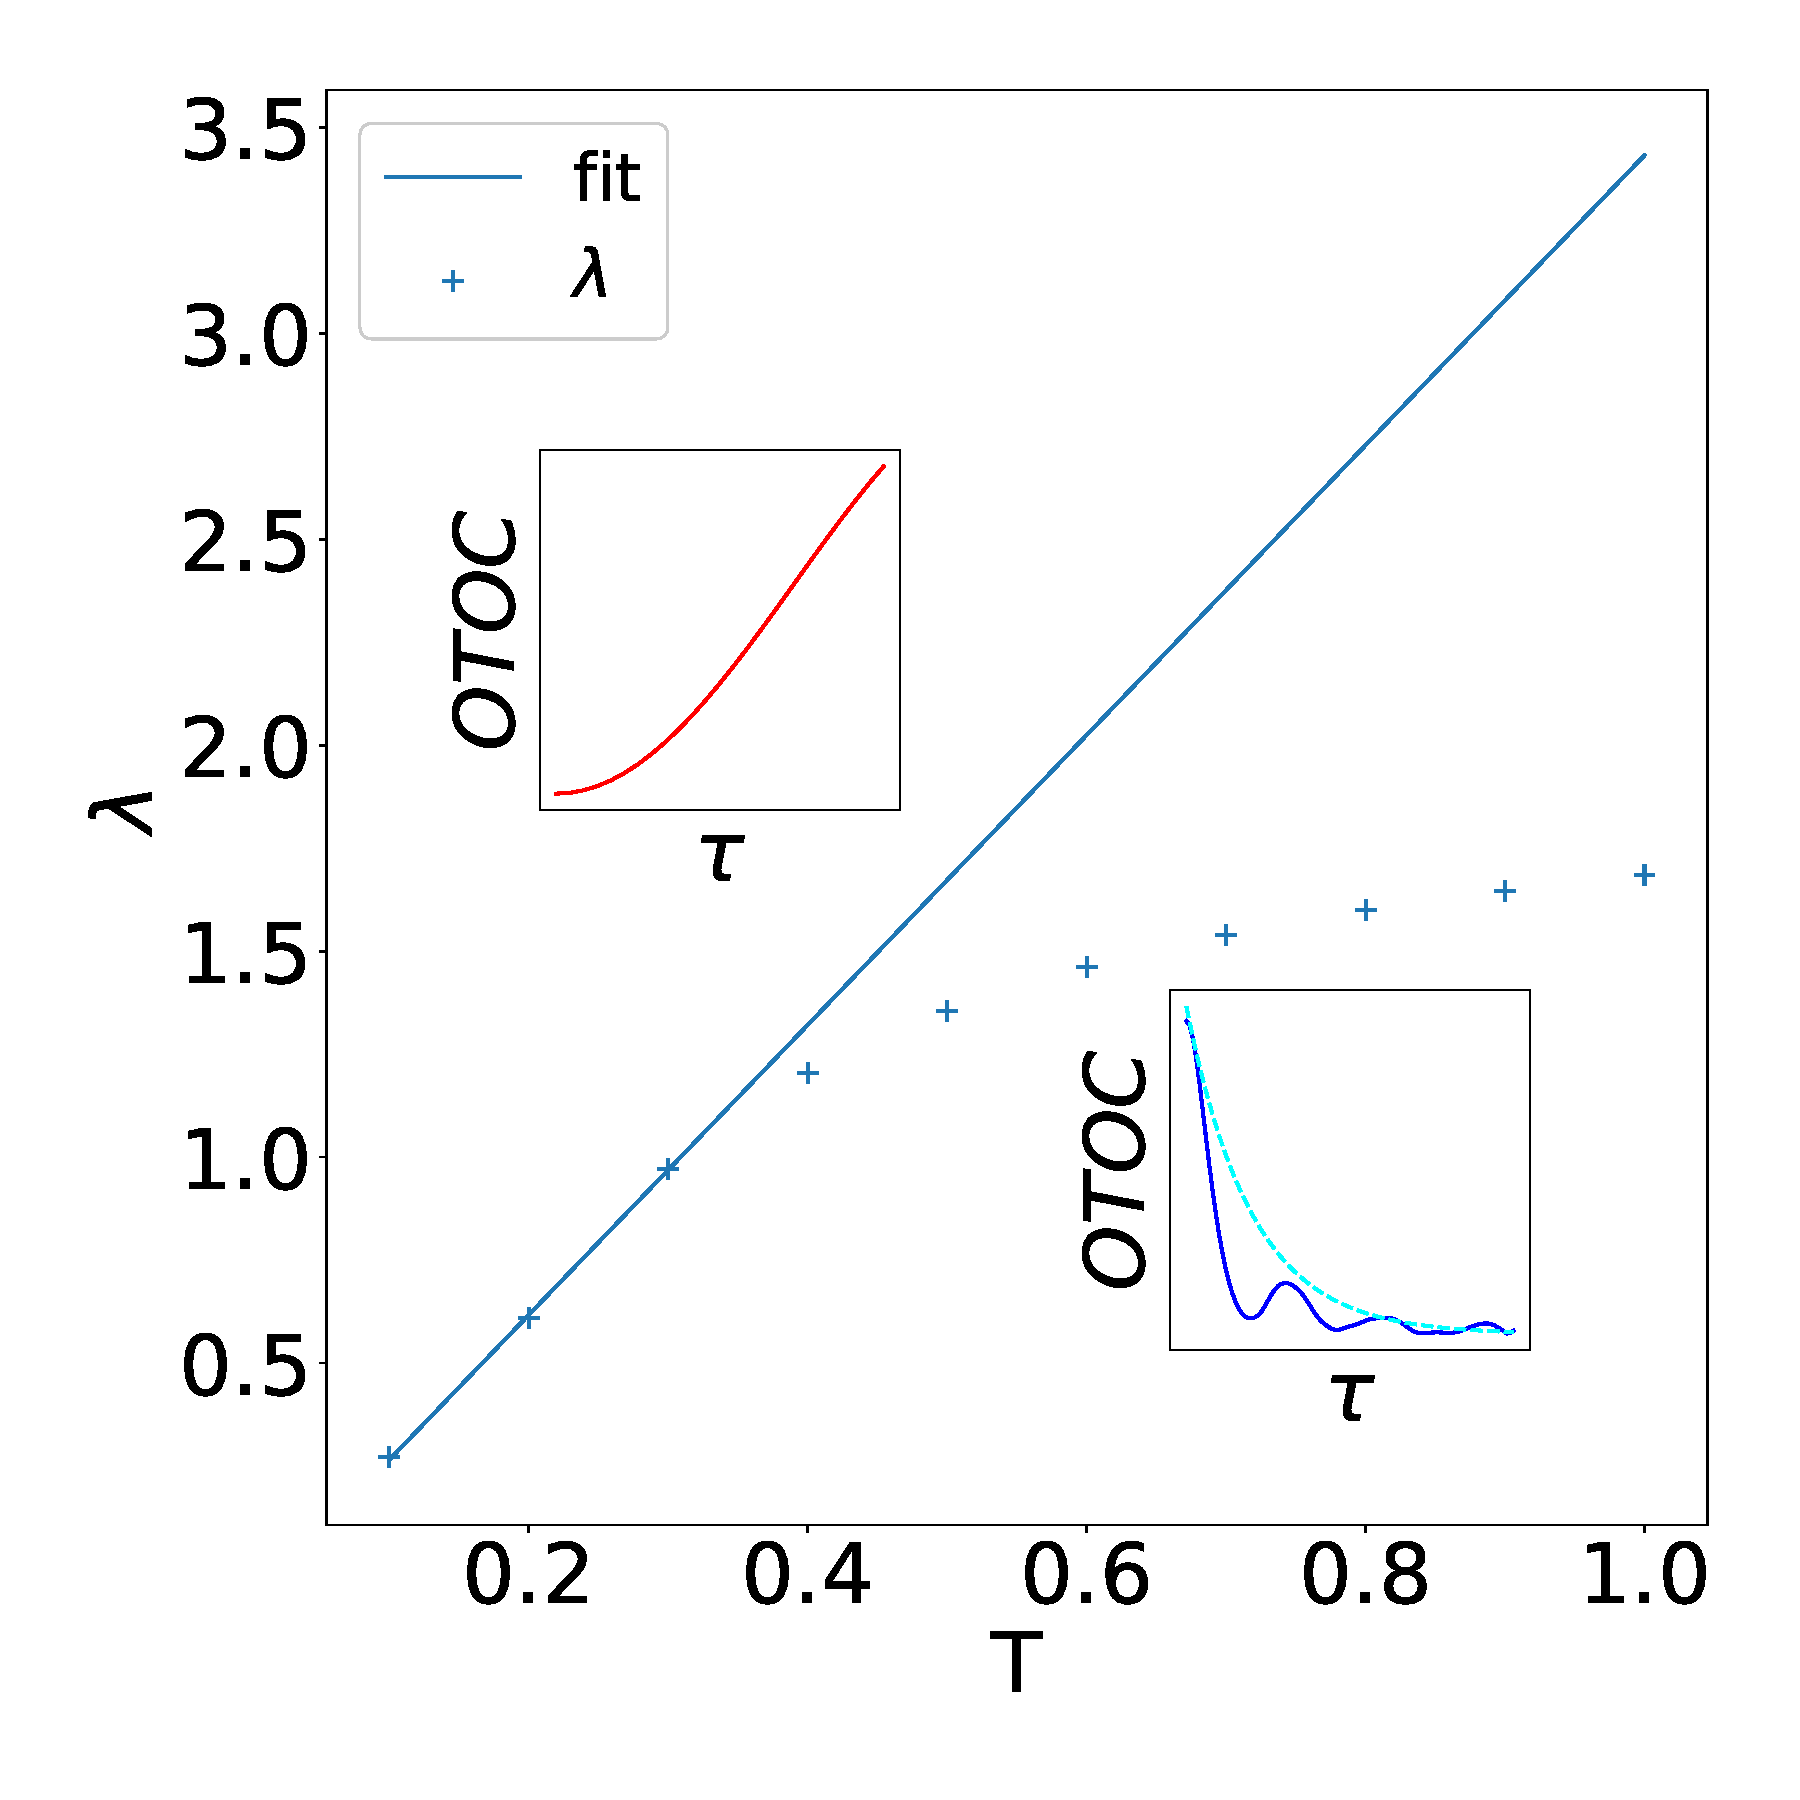
\includegraphics[width=\textwidth]{figs/SM/lambdaT.pdf}
    \begin{picture}(0,0)
    %{\def\unitlength{} \put(0.1\textwidth,1.1\textwidth){$(b)$}}
    {\def\unitlength{} \put(0.4\textwidth,0.97\textwidth){\scriptsize maximal}}
    {\def\unitlength{} \put(0.4\textwidth,0.92\textwidth){\scriptsize quantum chaos}}
    {\def\unitlength{} \put(0.34\textwidth,0.78\textwidth){\scriptsize SM}}
    {\def\unitlength{} \put(0.71\textwidth,0.48\textwidth){\scriptsize SC}}
    \end{picture}
    % \phantomsubcaption{\label{Lyapunov}}
    \end{minipage}
    %%%%%%%%%%%%%%%%%%%%%%%%%%%%%%%%%%%
    \begin{minipage}{0.49\linewidth}
    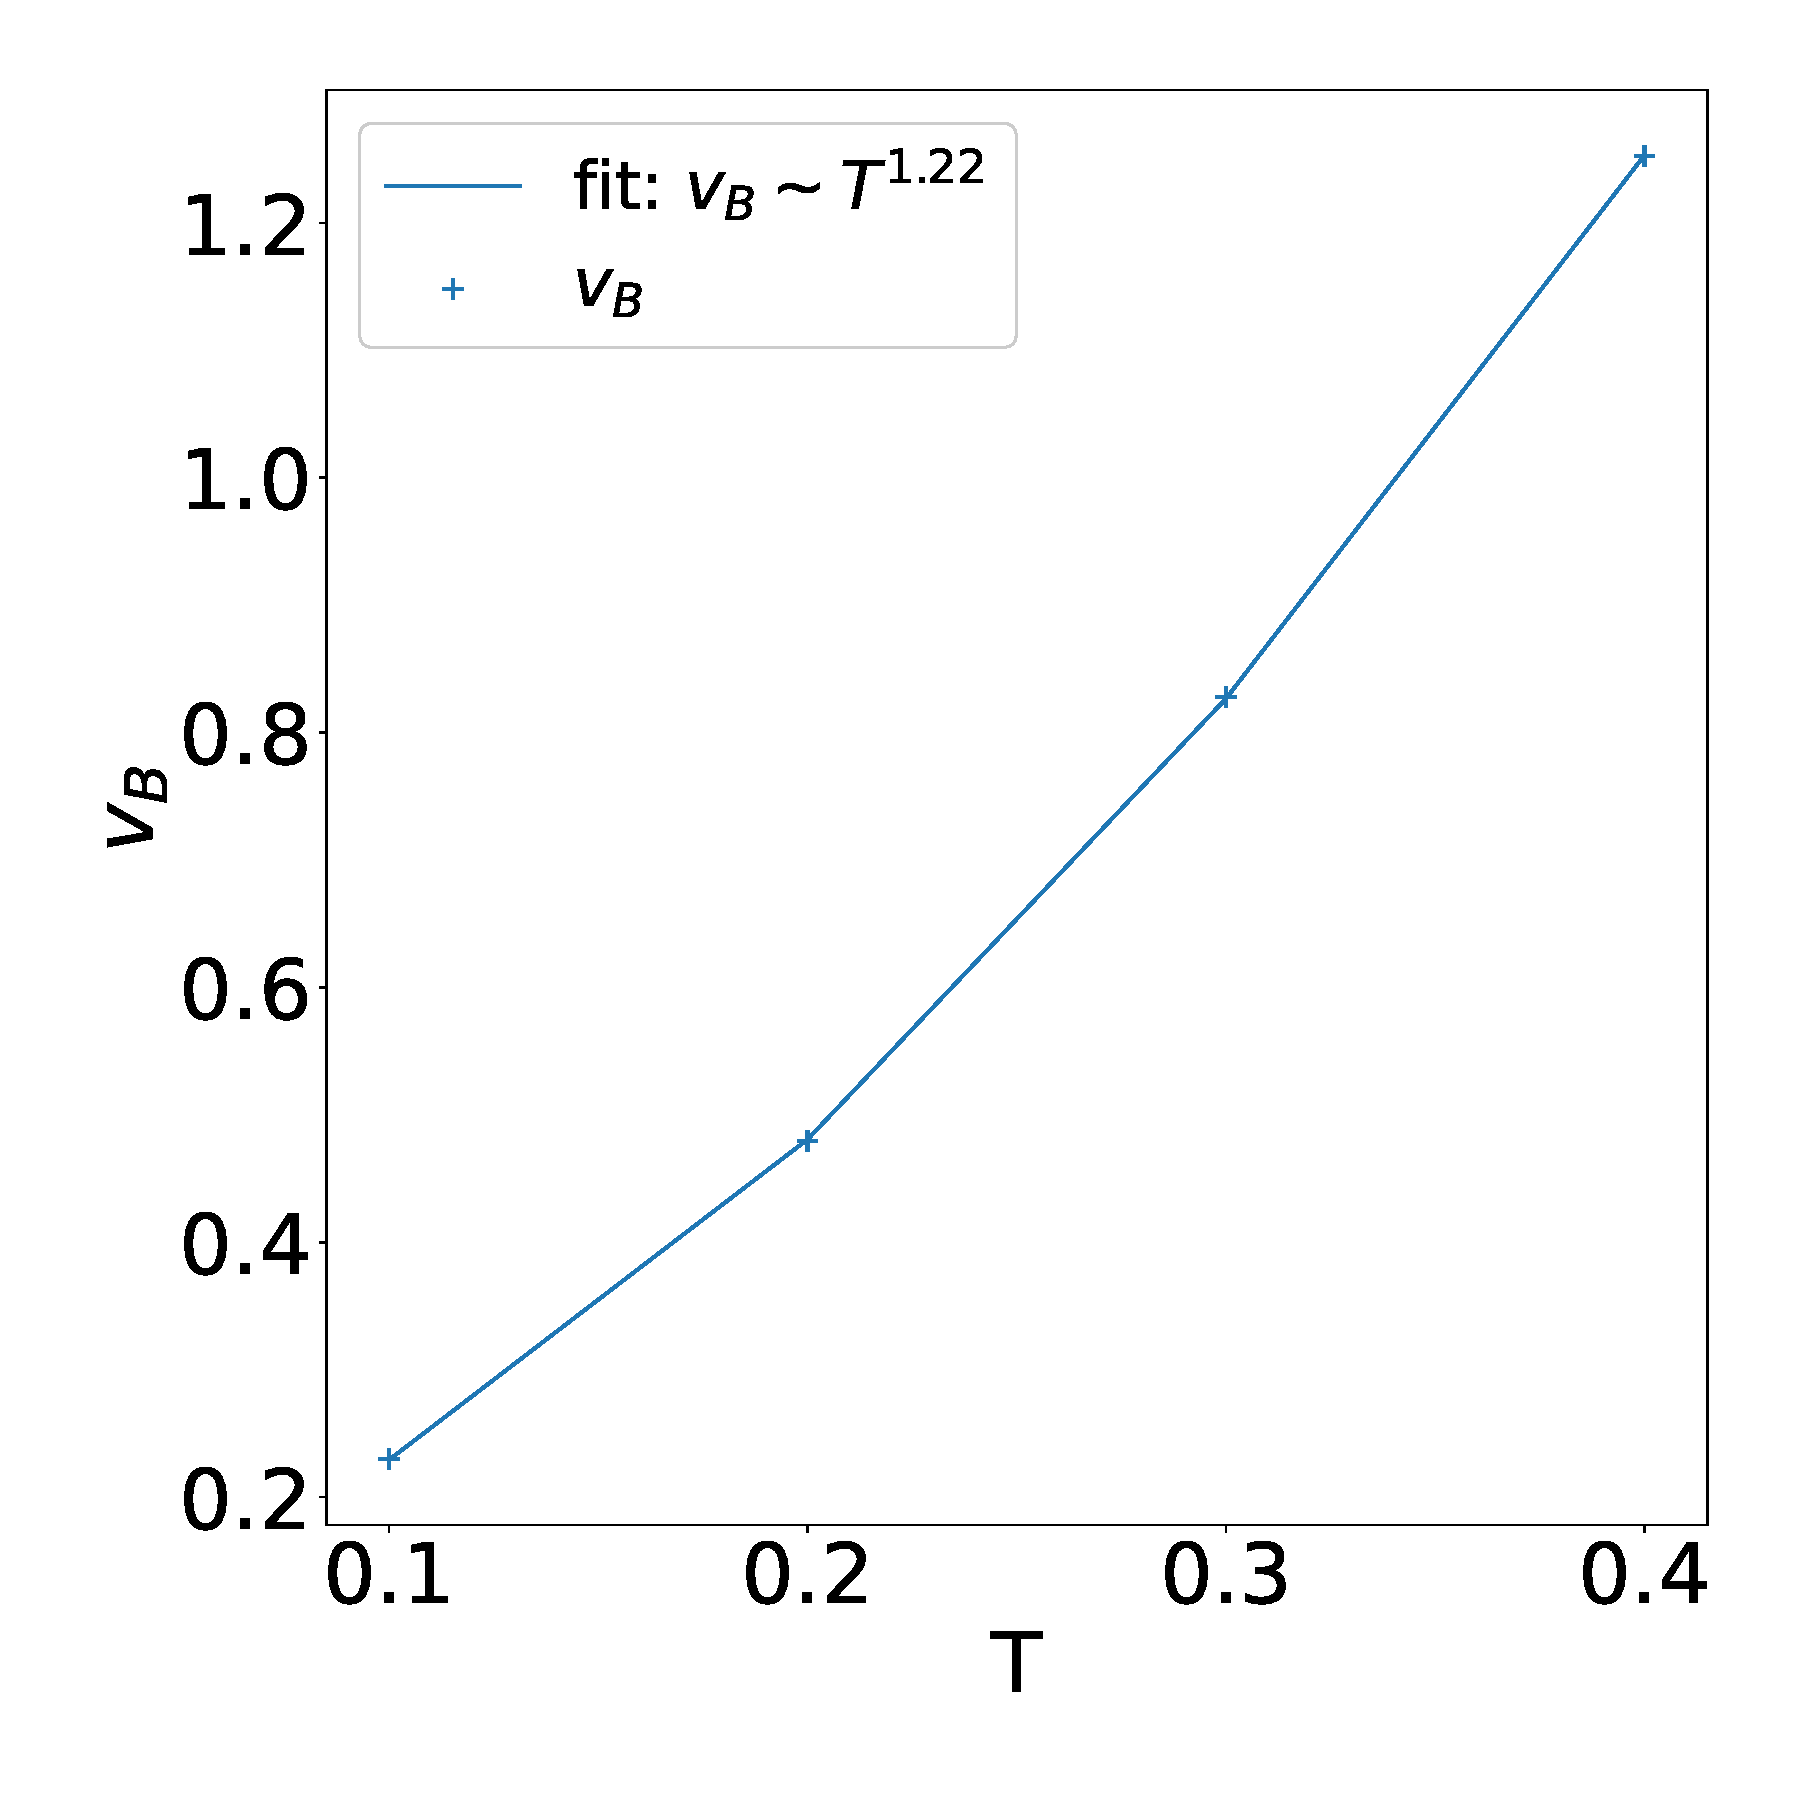
\includegraphics[width=\textwidth]{figs/SM/vB.pdf}
    \begin{picture}(0,0)
    % {\def\unitlength{} \put(0.1\textwidth,1.1\textwidth){$(c)$}}
    {\def\unitlength{} \put(0.21\textwidth,0.8\textwidth){\scriptsize information}}
    {\def\unitlength{} \put(0.21\textwidth,0.75\textwidth){\scriptsize scrambling}}
    \end{picture}
    % \phantomsubcaption{\label{vB}}
    \end{minipage}
\end{figure}
\end{column}
\end{columns}
\end{frame}
%----------------------------------------------------------------------------------------
\begin{frame}{Absence of zero-bias anomaly}
\begin{columns}
\begin{column}{0.5\textwidth}
\begin{figure}
    \centering
    \begin{minipage}{0.8\linewidth}
    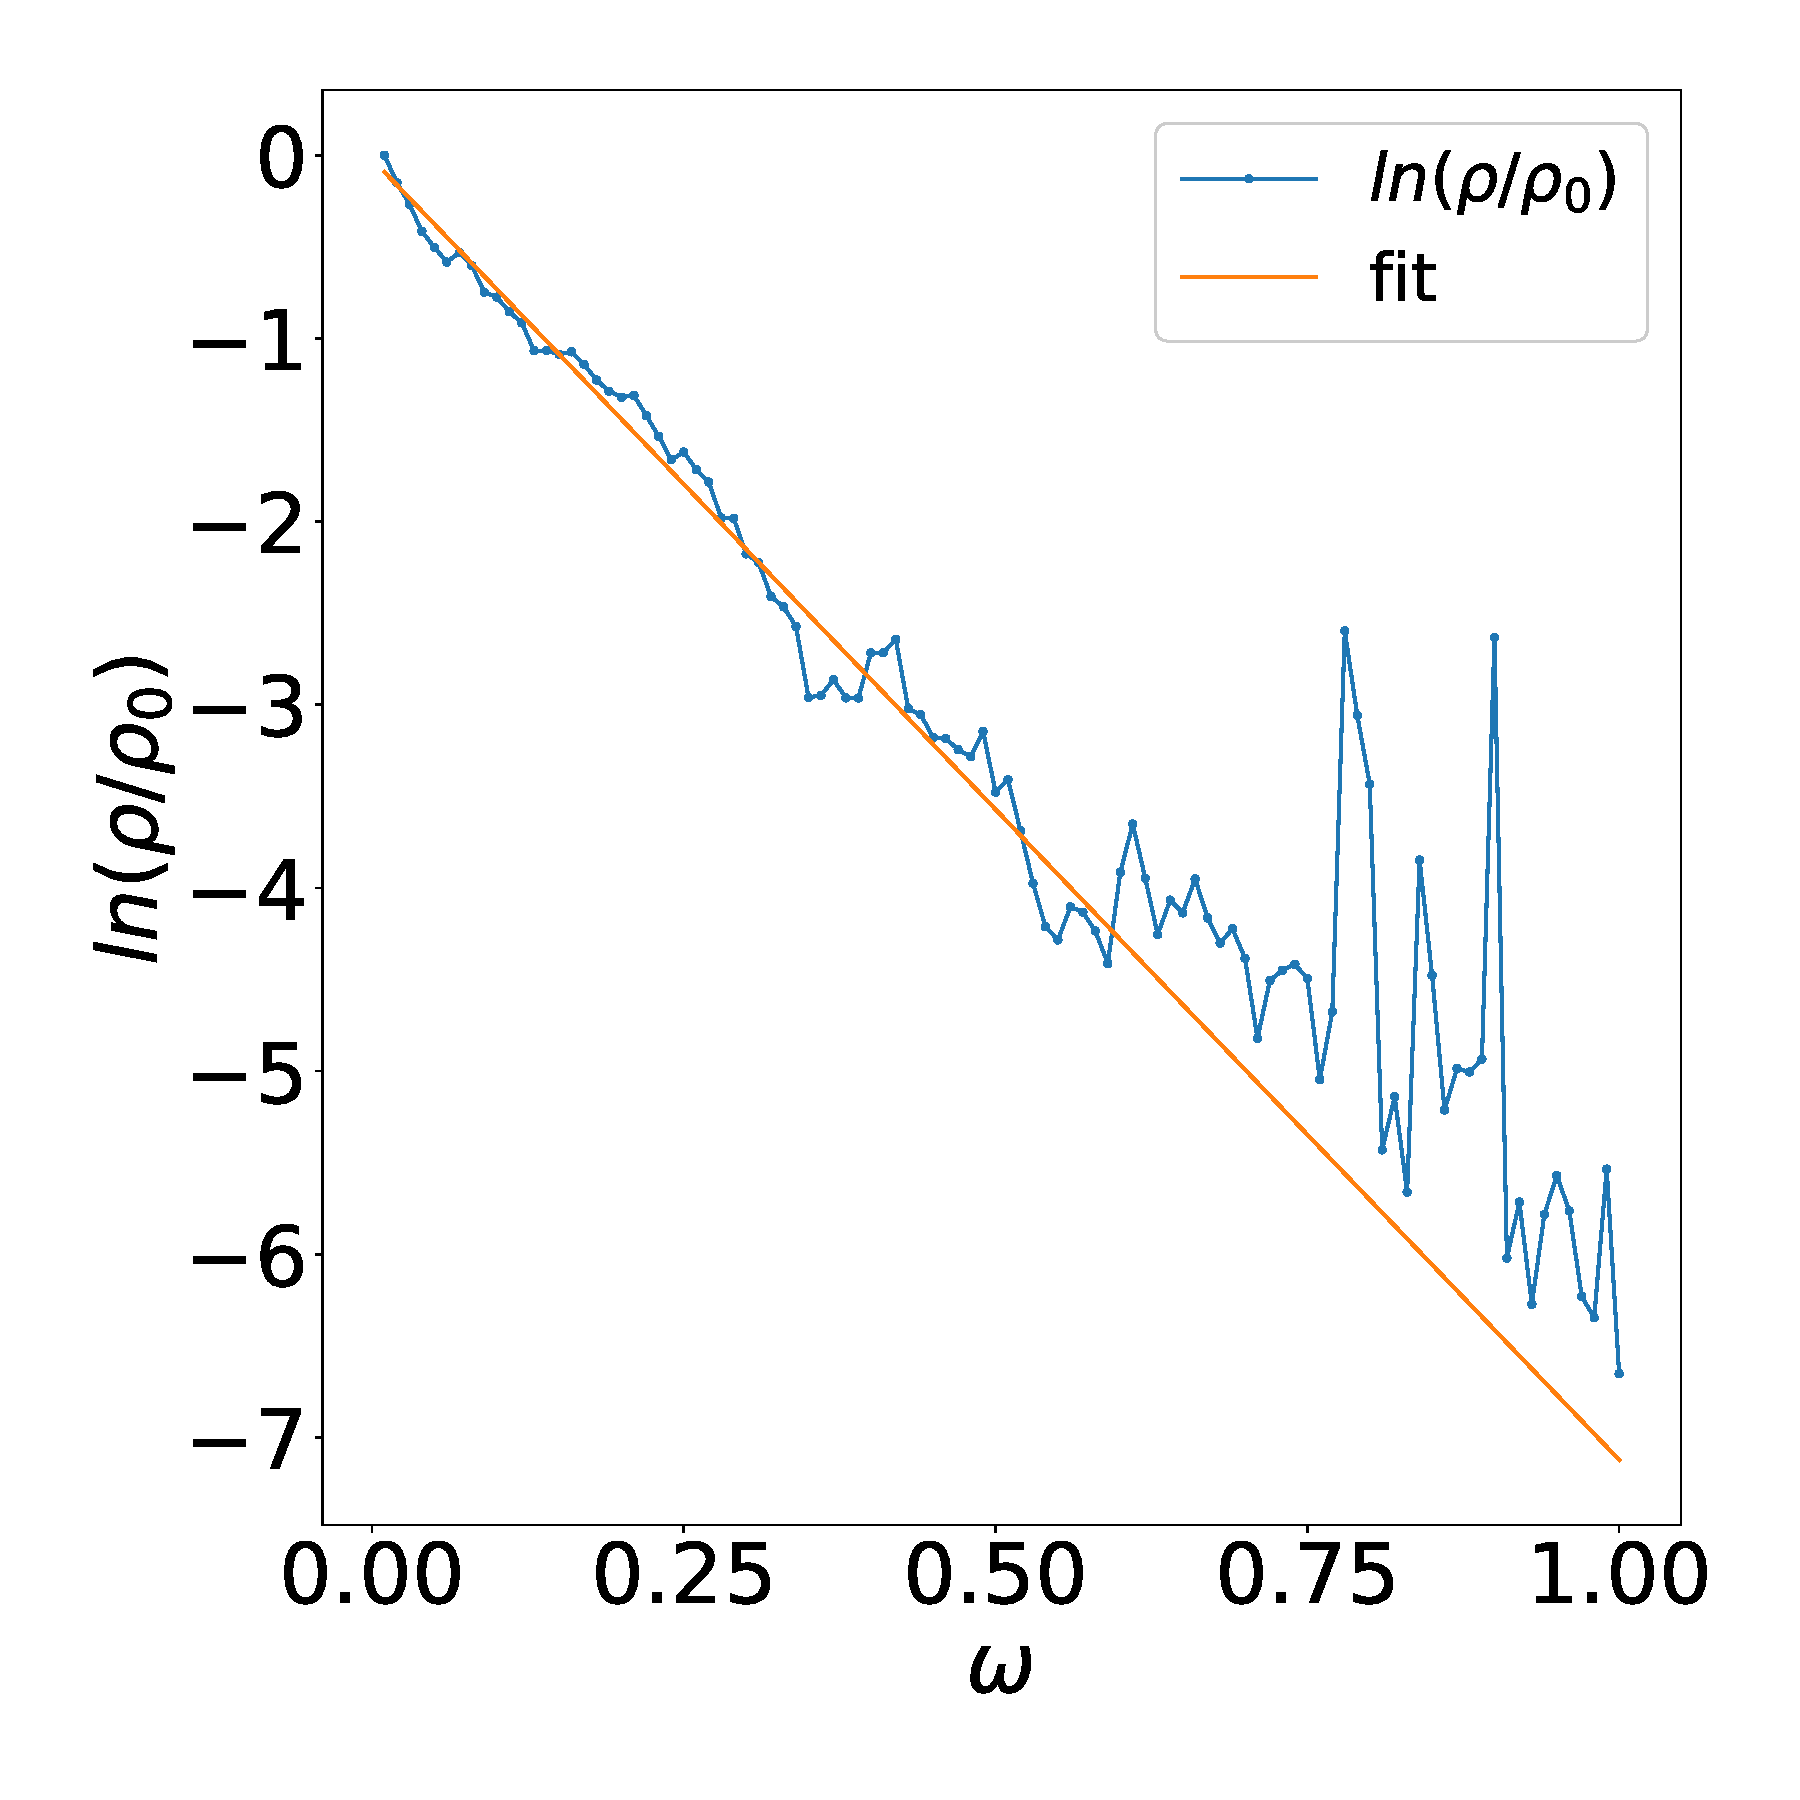
\includegraphics[width=\textwidth]{figs/SM/rho.pdf}
    \begin{picture}(0,0)
    %{\def\unitlength{} \put(0.1\textwidth,1.1\textwidth){$(d)$}}
    {\def\unitlength{} \put(0.21\textwidth,0.37\textwidth){\scriptsize absence of}}
    {\def\unitlength{} \put(0.21\textwidth,0.32\textwidth){\scriptsize zero-bias}}
    {\def\unitlength{} \put(0.21\textwidth,0.27\textwidth){\scriptsize anomaly}}
    \end{picture}
    % \phantomsubcaption{\label{rho}}
    \end{minipage}
\end{figure}
\end{column}

\setcounter{footnote}{11} % manually set the footnote counter
\begin{column}{0.5\textwidth}
\begin{itemize}
    \item For Fermi liquid, cancelling interference Friedel oscillation \\ $\implies$ logarithmic zero bias tunneling density anomaly \footnote[frame]{\cite{rudin1997tunneling,mariani2007zero,sedrakyan2007zero}}
    \item Absence of zero bias anomaly \\ $\implies$ lacking of quasiparticles
\end{itemize}
\end{column}
\end{columns}
\end{frame}
%----------------------------------------------------------------------------------------
\subsection{Phase diagram}
%----------------------------------------------------------------------------------------
\begin{frame}{Phase diagram}
\begin{columns}
\begin{column}{0.5\textwidth}
\begin{figure}
    \centering
    \begin{minipage}{\linewidth}
    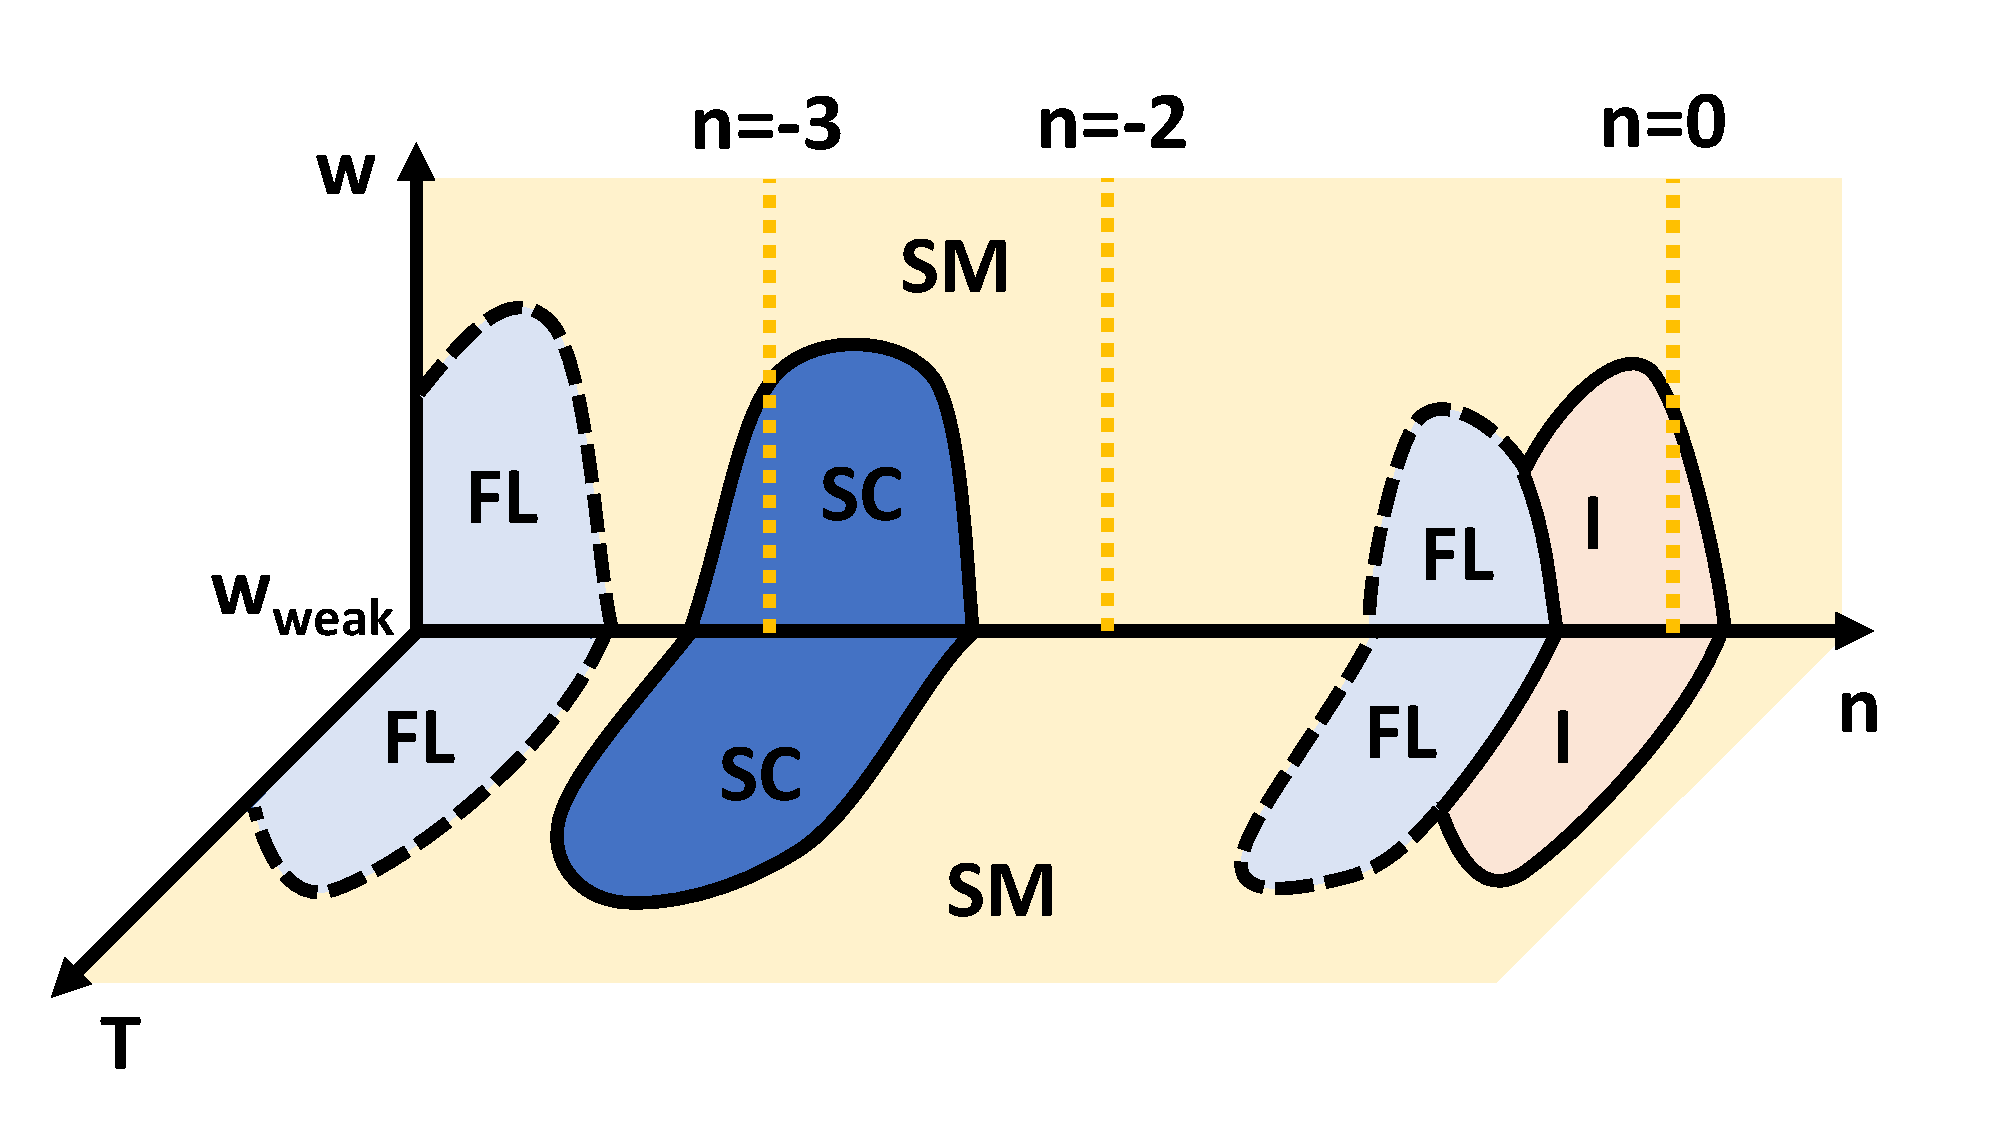
\includegraphics[width=\textwidth]{figs/SM/phase_diagram.pdf}
    % \begin{picture}(0,0)
    % {\def\unitlength{} \put(0.1\textwidth,1.1\textwidth){$(a)$}}
    % \end{picture}
    % \phantomsubcaption{\label{phase}}
    \end{minipage}
\end{figure}
\end{column}

\begin{column}{0.5\textwidth}
    \begin{itemize}
        \item Disordered MATBG can be effectively described by weakly coupled SYK bundles
        \item Strongly disordered MATBG shows quantum chaos and information scrambling
        \item Weakly disordered MATBG becomes the onset of superconductivity
        \item Phase diagram proposed base on the findings
    \end{itemize}
\end{column}
\end{columns}
\end{frame}